\documentclass{article}
\author{Max Carlson}
\usepackage{amsmath}
\usepackage{listings}
\usepackage{color}
\setlength\parindent{24pt}
\lstset{frame=tb,
	language=Python,
	aboveskip=3mm,
	belowskip=3mm,
	showstringspaces=false,
	columns=flexible,
	basicstyle={\small\ttfamily},
	numbers=none,
	numberstyle=\tiny\color{gray},
	keywordstyle=\color{blue},
	commentstyle=\color{dkgreen},
	stringstyle=\color{mauve},
	breaklines=true,
	breakatwhitespace=true,
	tabsize=3}

\usepackage{graphicx}
\graphicspath{.}
\usepackage{geometry}
%\usepackage{float}
\geometry{paperheight=11.0in}%
\geometry{paperwidth=8.5in}%
\geometry{textwidth=6.0in}%
\geometry{left=1.125in}  %{(\paperwidth-\textwidth)/2)}
\geometry{right=1.125in}  %{(\paperwidth-\textwidth)/2)}

\title{Machine Learning Programming 2}
\begin{document}
	\maketitle
	
	The Naive Bayes Classifier works by assigning probabilities to different outcomes for new data based on the features of the training data. In order to create a Naive Bayesian Classifier, one needs to compute the prior probabilities for each class, as well as the likelihoods. Because we had continuous valued features, we made the assumption that the data was normally distributed and used $P(x_i|c_j) = N(x_i;\mu _{i,c_j},\sigma_{i,c_j})=\frac{1}{\sqrt{2\pi}\sigma}e^{-(\frac{(x-\mu)^2}{2\sigma^2})}$ to calculate the likelihoods. In order to find the likelihoods, I had to calculate the mean and standard deviations of each feature in the training dataset. Once the priors and the likelihoods have been calculated using the training data, one can classify new data using the following method: \\
	
	$class_{NB}(x)=\underset{class}{argmax}\log[P(class)\prod_{i}^{}P(x_i|class)]$
	\\
	
	The data was split into two, a training and a test dataset. The data was randomized first, then split 50/50 training/test, keeping similar ratio of spam/not spam during the split. After training, the accuracy of the classifier on the test dataset was 88.6\%, the precision was 89.7\%, and the recall was 80.4\%. We make the assumption that the features are all fully independent, but I doubt that is the case. In spite of that, we do relatively well here with close to 90\% accuracy. Possibly enough of the features are independent *enough* for our naive implementation to deliver good results. Or perhaps we don't need independent features, we only need features that correlate with a particular state (spam/not spam) and the naive assumption greatly simplifies (or makes possible) estimating these probabilities.
	
	
	\begin{figure}[]
		\begin{center}
			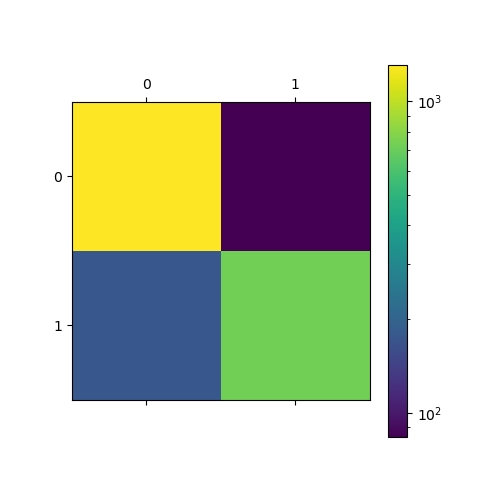
\includegraphics[]{confusion.png}		
			\caption{Confusion Matrix for test dataset}	\label{fig:xray}
		\end{center}
	\end{figure}
\end{document}